\documentclass[../characterization.tex]{subfiles}
\graphicspath{{\subfix{../../../../images/}}}
\begin{document}
    \textbf{Transmission Electron Microscopy (TEM)}\cite{b13} is an advanced imaging and analytical technique used to study 
    the internal structure, crystallography, and composition of materials at the nanoscale. It provides 
    high-resolution images and enables detailed analysis of the morphology, crystal structure, defects, and 
    interfaces of nanophosphors.
    \begin{Figure}
        \centering
        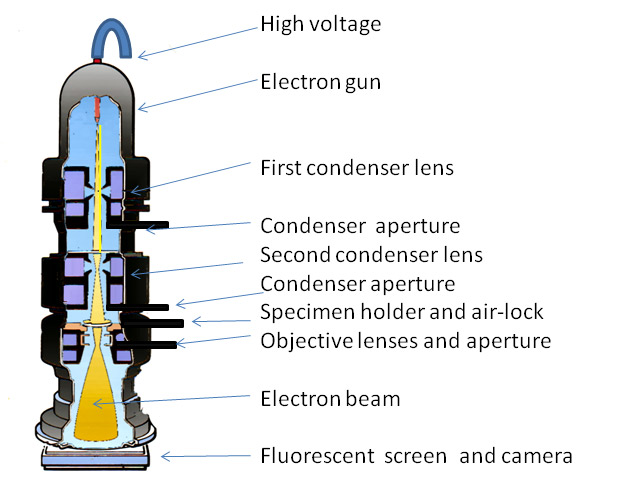
\includegraphics[width=0.6\linewidth]{tem.jpg}
        \captionof{figure}{Schematic diagram of Transmission Electron Microscope\cite{u13}}\label{fig:tem}
    \end{Figure}
    TEM uses a focused beam of electrons that passes through an ultra-thin sample. The electron beam is 
    generated from an electron source, such as a tungsten filament or field emission gun, and accelerated to 
    high energy. To perform TEM analysis, the nanophosphor sample needs to be prepared as thin specimens with 
    thicknesses typically ranging from tens to hundreds of nanometers. The most common technique for sample 
    preparation is known as \"thinning by mechanical polishing\" or using specialized equipment like a focused 
    ion beam (FIB) system. The electron beam passes through the sample, and the transmitted electrons are 
    collected and focused onto a fluorescent screen or a charge-coupled device (CCD) camera. The resulting 
    image represents the transmitted electron intensity, providing a projection of the sample's internal structure.It 
    allows for high-resolution imaging of the sample, providing details at the atomic level. It enables the 
    observation of lattice fringes, defects, grain boundaries, and other fine structural features of the 
    nanophosphor.
    \\
    TEM is a powerful tool for nanophosphor characterization, offering exceptional spatial resolution and the 
    ability to study the nanoscale structure and properties of materials. It enables researchers to investigate 
    the internal structure, defects, and interfaces of nanophosphors, contributing to a deeper understanding of 
    their properties and guiding their development for various applications.
\end{document}